\section{Technical Implementation}

% Do these need references?
Discovery Service is implemented with Python programming language and Flask Web framework. They were chosen because all of the components in Cloudify are also written in Python and Flask is used primarily for providing REST APIs. Even though Discovery Service does not provide any REST APIs, Flask is used for configuration management and source code organisation. Naturally, if need arises in the future to expand Discovery Service with a REST API, the development work is streamlined because of the framework.

In addition to Python program, Discovery Service relies on Redis \cite{Redis} as an in-memory key-value storage. Redis is a completely separate process in addition to Discovery Service. The preferred way of deploying Redis is in a docker container as it doesn't require installation or configuration save for exposing a correct port in the container and specifying Redis' address to Discovery Service. Redis could also be installed in the host system or even a remote system, though latter option has no practical purpose due to network latency as Redis achieves its high performance by storing values in the memory instead of disk.

\begin{figure}[ht!]
\centering
  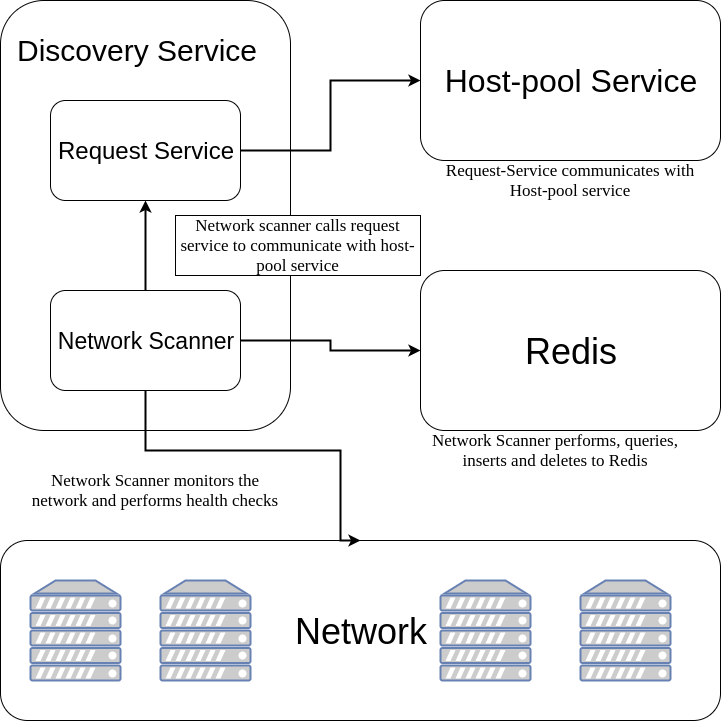
\includegraphics[width=12cm,height=12cm, keepaspectratio]{Discovery-service-communication.png}
  \caption{The communication relationships between Discovery Service and other components}
  \label{fig:communications}
\end{figure}

On the source code level, Discovery Service consists of two major components: The network scanner and request service. The network scanner is given a subnet as a parameter and it constantly sniffs the network detecting joining and already present devices and keeping track of them. Its other task is to periodically send health checks to known devices and if a health check fails enough times, it removes the given device from the logical host pool. Request service is responsible for sending HTTP requests to the Cloudify Host-pool service. It is called by the request service and it runs asynchronously. In addition to HTTP requests, it performs checks to ensure that the state of Discovery service's and Host-pool service's databases correlate.

The communication relationships between different components in the system are depicted in figure \ref{fig:communications}. The source code for Discovery Service as well as the documentation can be found at \url{https://bitbucket.org/Fleuri/discoveryserviceforcloudify/src/master/}

\subsection{Network Scanner}

The Network Scanner has two main functions, sniffer and pinger, and they run concurrently on two threads. Sniffer listens to ARP packets in the network and upon receiving one, stores the details of the sender device. Pinger function periodically sends ARP pings to previously discovered device and keeps track of their successes, eventually removing unresponsive devices from the logical host pool. In addition to two main functions there's a startup function that initialises both local Redis storage and the Host-pool service's database. It pings all of the IP addresses in the given IP range and stores the found device details to databases.

\subsubsection{Sniffer}

Sniffer is started in its own thread during the start up sequence of the Discovery Service. It uses \textit{Scapy} library \cite{scapy} for Python. Sniffer function is given three arguments: 

\begin{enumerate}
\item \textbf{The network interface} which the Sniffer listens to for incoming packets.
\item \textbf{The callback function} which details further instructions to perform when a packet is caught.
\item \textbf{The filter} which restricts the type of packets caught.
\end{enumerate}

Only the interface can be set by the user of the Discovery Service. The callback function is the core application logic of the sniffer and the Discovery Service itself relies on sniffing ARP packets and therefore the filter is set accordingly.

When it comes to programming logic, the callback function is the most interesting part of the sniffer. Its purpose is to evaluate whether an ARP request comes from a new or know device and store details about them. When the function receives an ARP packet it first filters out packets that are not standard ARP requests. There are two such cases: ARP Probe \cite{rfc5227}, in which the source IP address or hardware address of the ARP request is \textit{0.0.0.0} or \textit{00:00:00:00:00:00} respectively, and gratuitous ARP in which the hardware address is \textit{ff:ff:ff:ff:ff:ff}. The user can also define a list of IP and hardware addresses which the Discovery Service should ignore i.e. devices on which Cloudify should not run workloads. Such devices include the host on which Cloudify manager runs and network devices such as routers.

Next the function checks whether the packet's origin is an already known host by querying Redis. If the host is not previously known, the function starts a new thread to add the host to the Host-pool service. See section \ref{requestservice}.

Whether the packet's

\subsubsection{Pinger}

\subsection{Request Service} \label{requestservice}

